\documentclass[conference,10pt]{IEEEtran}

\usepackage[utf8]{inputenc}
\usepackage[T1]{fontenc}
\usepackage{booktabs}
\usepackage{amsmath}
\usepackage{amssymb}
\usepackage{xcolor}
\usepackage{multirow}
\usepackage{graphicx}
\usepackage{hyperref}
\usepackage{pgfplots}
\pgfplotsset{compat=1.18}
\usepgfplotslibrary{fillbetween}
\usetikzlibrary{patterns,patterns.meta}
\usepackage{subcaption}

% Paul Tol High Contrast palette — colour-blind & grayscale safe
\definecolor{ptblue}{HTML}{004488}
\definecolor{ptgold}{HTML}{DDAA33}
\definecolor{ptrose}{HTML}{BB5566}
\definecolor{ptblack}{HTML}{000000}
\definecolor{ptgray}{HTML}{AAAAAA}

% IEEE-style axis defaults (klb2/betterplot-inspired)
\pgfplotsset{
  every axis/.append style={
    xlabel near ticks,
    ylabel near ticks,
    grid style={line width=.25pt, draw=gray!30},
    minor grid style={line width=.1pt, draw=gray!20},
    legend cell align=left,
  },
}

% Stub out \cite so it doesn't error on missing .bib
\renewcommand{\cite}[1]{[#1]}

% tablenotes: render as a compact list below the tabular
\newenvironment{tablenotes}{%
  \par\vskip4pt\begin{list}{}{\footnotesize\setlength{\leftmargin}{0pt}%
    \setlength{\itemsep}{0pt}\setlength{\parsep}{0pt}%
    \setlength{\topsep}{0pt}\setlength{\partopsep}{0pt}}%
}{%
  \end{list}\vskip2pt
}

\begin{document}

\title{Secure-Tunnel: Post-Quantum Cryptographic Overlay\\for UAV C2 Links\\
{\normalsize Results and Analysis Section --- v4.0 (Cross-Axis Interactions)}}
\author{Draft compilation for review}
\maketitle

% IEEE VTC Fall 2026 — Results and Analysis [v4.0]
% Data: v2-1.8ghz (KEM/SIG, 100 iter, 1 kHz INA219)
%       vtc-fall-aead-rerun (AEAD, 10k iter, ~100 Hz INA219, native C Ascon)
%       bench_ddos_results (72 suites x 3 detectors)
%       isorc2026 cross-axis AEAD×DDoS measurements
% Platform: RPi4B Rev 1.5, BCM2711, Cortex-A72 @ 1.8 GHz, 4 GB, Debian 12

\section{Results and Analysis}
\label{sec:results}

All measurements were collected on a Raspberry Pi~4 Model~B Rev~1.5
(BCM2711, four Cortex-A72 cores at 1.8\,GHz, 4\,GB RAM) running
Debian~12 (kernel 6.12.47) with the \texttt{performance} CPU governor.
Timing used \texttt{time.perf\_counter\_ns()} with garbage collection
disabled; power was sampled via an INA219 current sensor
(0.1\,$\Omega$ shunt, $V_\text{BUS}$ gain correction~1.22) at up
to 1\,kHz.  Idle power: $P_\text{idle} = 3.32$\,W (30\,s baseline).
The Cortex-A72 lacks ARMv8 Crypto Extensions; AES-GCM therefore
executes in software table-lookup mode, while ChaCha20-Poly1305
exploits 128-bit NEON SIMD.
PQC primitives: liboqs-python~0.14.0.
AEAD ciphers: OpenSSL~3.5.4 (AES-256-GCM, ChaCha20-Poly1305),
ascon-c v1.2 opt64 via \texttt{ctypes} (Ascon-128a, KAT-verified).
Table~\ref{tab:aliases} defines the short aliases used throughout.

\begin{table}[t]
\centering
\caption{Algorithm Aliases and NIST Security Levels}
\label{tab:aliases}
\footnotesize
\begin{tabular}{@{}llcl@{}}
\toprule
\textbf{Alias} & \textbf{Full Name} & \textbf{Level} & \textbf{Type} \\
\midrule
ML512  & ML-KEM-512                & L1 & KEM  \\
ML768  & ML-KEM-768                & L3 & KEM  \\
ML1024 & ML-KEM-1024               & L5 & KEM  \\
HQ128  & HQC-128                   & L1 & KEM  \\
HQ192  & HQC-192                   & L3 & KEM  \\
HQ256  & HQC-256                   & L5 & KEM  \\
MC348  & Classic-McEliece-348864   & L1 & KEM  \\
MC460  & Classic-McEliece-460896   & L3 & KEM  \\
MC8192 & Classic-McEliece-8192128  & L5 & KEM  \\
\midrule
DSA44  & ML-DSA-44                 & L1 & SIG  \\
DSA65  & ML-DSA-65                 & L3 & SIG  \\
DSA87  & ML-DSA-87                 & L5 & SIG  \\
F512   & Falcon-512                & L1 & SIG  \\
F1024  & Falcon-1024               & L5 & SIG  \\
SP128  & SPHINCS$^+$-SHA2-128s     & L1 & SIG  \\
SP192  & SPHINCS$^+$-SHA2-192s     & L3 & SIG  \\
SP256  & SPHINCS$^+$-SHA2-256s     & L5 & SIG  \\
\midrule
AESG   & AES-256-GCM               & ---& AEAD \\
CH20   & ChaCha20-Poly1305         & ---& AEAD \\
ASC    & Ascon-128a                & ---& AEAD \\
\bottomrule
\end{tabular}
\end{table}

% =====================================================================
\subsection{Primitive-Level Performance}
\label{sec:primitive}

\textbf{Key Encapsulation.}\quad
Fig.~\ref{fig:kem_cost} and Table~\ref{tab:kem} compare nine KEM
algorithms across three NIST security levels (100~iterations,
1\,kHz INA219).  Each cycle comprises keygen, encapsulation, and
decapsulation---all three are executed per rekey event.
Fig.~\ref{fig:primitive_cost} presents both KEM and signature
results using consistent log-scale grouping.

\begin{figure}[t]
\centering
\begin{subfigure}[b]{\columnwidth}
\centering
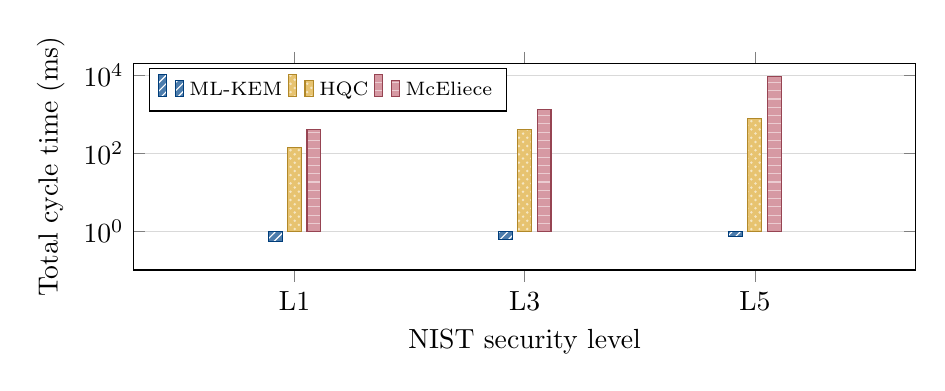
\begin{tikzpicture}
\begin{axis}[
  width=.95\columnwidth,
  height=4.2cm,
  ybar,
  bar width=5pt,
  ymode=log,
  ylabel={Total cycle time (ms)},
  symbolic x coords={L1, L3, L5},
  xtick=data,
  xlabel={NIST security level},
  ymin=0.1, ymax=20000,
  legend style={at={(0.02,0.98)},anchor=north west,font=\scriptsize,
    legend columns=3},
  ymajorgrids=true,
  enlarge x limits=0.35,
]
\addplot[fill=ptblue!70, draw=ptblue!90!black,
  postaction={pattern=north east lines, pattern color=white}]
  coordinates {(L1,0.550) (L3,0.604) (L5,0.720)};
\addplot[fill=ptgold!70, draw=ptgold!80!black,
  postaction={pattern=crosshatch dots, pattern color=ptgold!30}]
  coordinates {(L1,140.4) (L3,415.4) (L5,767.2)};
\addplot[fill=ptrose!60, draw=ptrose!80!black,
  postaction={pattern=horizontal lines, pattern color=ptrose!30}]
  coordinates {(L1,407.4) (L3,1371) (L5,9233)};
\legend{ML-KEM, HQC, McEliece}
\end{axis}
\end{tikzpicture}
\caption{KEM: keygen + encaps + decaps}
\label{fig:kem_cost}
\end{subfigure}
\vspace{2pt}
\begin{subfigure}[b]{\columnwidth}
\centering
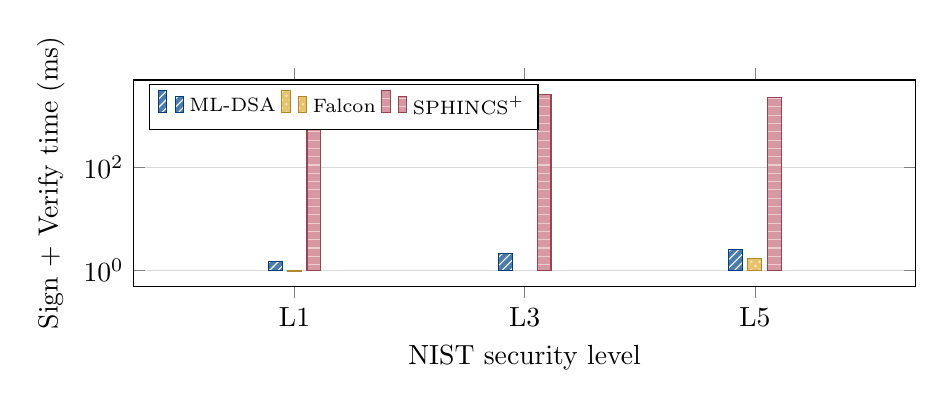
\begin{tikzpicture}
\begin{axis}[
  width=.95\columnwidth,
  height=4.2cm,
  ybar,
  bar width=5pt,
  ymode=log,
  ylabel={Sign + Verify time (ms)},
  symbolic x coords={L1, L3, L5},
  xtick=data,
  xlabel={NIST security level},
  ymin=0.5, ymax=5000,
  legend style={at={(0.02,0.98)},anchor=north west,font=\scriptsize,
    legend columns=3},
  ymajorgrids=true,
  enlarge x limits=0.35,
]
\addplot[fill=ptblue!70, draw=ptblue!90!black,
  postaction={pattern=north east lines, pattern color=white}]
  coordinates {(L1,1.510) (L3,2.117) (L5,2.570)};
\addplot[fill=ptgold!70, draw=ptgold!80!black,
  postaction={pattern=crosshatch dots, pattern color=ptgold!30}]
  coordinates {(L1,0.970) (L5,1.732)};
\addplot[fill=ptrose!60, draw=ptrose!80!black,
  postaction={pattern=horizontal lines, pattern color=ptrose!30}]
  coordinates {(L1,1469.6) (L3,2612.3) (L5,2324.3)};
\legend{ML-DSA, Falcon, SPHINCS$^+$}
\end{axis}
\end{tikzpicture}
\caption{SIG: sign + verify (Falcon unavailable at L3)}
\label{fig:sig_cost}
\end{subfigure}
\caption{Primitive-level computational cost by NIST level (log scale).
  ML-KEM and ML-DSA/Falcon complete in $<$\,3\,ms at all levels;
  SPHINCS$^+$ and McEliece are 2--4 orders of magnitude slower.}
\label{fig:primitive_cost}
\end{figure}

\begin{table}[t]
\centering
\caption{KEM Per-Operation Breakdown (100 iter, 1\,kHz INA219)}
\label{tab:kem}
\footnotesize
\setlength{\tabcolsep}{3pt}
\begin{tabular}{@{}lcrrrrr@{}}
\toprule
\textbf{Alias} & \textbf{Lvl} &
  \textbf{KeyGen} & \textbf{Encaps} & \textbf{Decaps} &
  \textbf{$E_\text{tot}$} &
  \textbf{$\rho$} \\
& & (ms) & (ms) & (ms) & ($\mu$J) & \\
\midrule
ML512  & L1 & 0.240 & 0.152 & 0.158 & 1\,907    & 1.00$\times$ \\
HQ128  & L1 & 22.33 & 44.68 & 73.39 & 535\,253  & 255$\times$ \\
MC348  & L1 & 351.0 & 0.466 & 55.98 & 1\,737\,186 & 741$\times$ \\
\midrule
ML768  & L3 & 0.237 & 0.182 & 0.185 & 2\,112    & 1.00$\times$ \\
HQ192  & L3 & 67.68 & 135.8 & 211.9 & 1\,651\,813 & 688$\times$ \\
MC460  & L3 & 1\,281 & 0.872 & 89.59 & 6\,025\,434 & 2\,272$\times$ \\
\midrule
ML1024 & L5 & 0.273 & 0.216 & 0.231 & 2\,507    & 1.00$\times$ \\
HQ256  & L5 & 124.4 & 250.2 & 392.6 & 3\,136\,867 & 1\,066$\times$ \\
MC8192 & L5 & 9\,021 & 1.894 & 210.1 & 40\,583\,491 & 12\,823$\times$ \\
\bottomrule
\end{tabular}
\begin{tablenotes}
\footnotesize
\item $E_\text{tot}$: total energy (keygen+encaps+decaps), INA219-measured.
  $\rho$: total cycle time relative to ML-KEM at same level.
\end{tablenotes}
\end{table}

ML-KEM completes a full cycle in under 0.72\,ms through Level~5,
drawing 3.46--3.48\,W.  HQC is 255--1\,066$\times$ slower, driven
by decapsulation (73--393\,ms).  Classic~McEliece exhibits extreme
keygen asymmetry: MC8192 requires 9.02\,s for keygen but only
1.89\,ms for encapsulation, making it feasible only with
pre-provisioned keys.

\medskip
\textbf{Digital Signatures.}\quad
Fig.~\ref{fig:sig_cost} and Table~\ref{tab:sig} evaluate eight
signature schemes.  Keygen is a one-time cost amortized over the
key lifetime (0.4--282\,ms); the per-handshake sign and verify
operations determine rekey latency.

\begin{table}[t]
\centering
\caption{Signature Runtime Cost: Sign + Verify (100 iter, 1\,kHz INA219).
  KeyGen is a one-time cost and excluded from $\rho$.}
\label{tab:sig}
\footnotesize
\begin{tabular}{@{}lcrrrrr@{}}
\toprule
\textbf{Alias} & \textbf{Lvl} &
  \textbf{Sign} & \textbf{Verify} &
  \textbf{$E_\text{s}$} & \textbf{$E_\text{v}$} &
  \textbf{$\rho$} \\
& & (ms) & (ms) & ($\mu$J) & ($\mu$J) & \\
\midrule
DSA44  & L1 & 1.179 & 0.331  & 4\,264  & 1\,175  & 1.00$\times$ \\
F512   & L1 & 0.778 & 0.192  & 2\,773  & 683     & 0.64$\times$ \\
SP128  & L1 & 1\,468 & 1.582  & 6\,008\,719 & 5\,690 & 972$\times$ \\
\midrule
DSA65  & L3 & 1.633 & 0.484  & 5\,849  & 1\,723  & 1.00$\times$ \\
SP192  & L3 & 2\,610 & 2.299  & 10\,628\,558 & 8\,318 & 1\,234$\times$ \\
\midrule
DSA87  & L5 & 1.847 & 0.723  & 6\,612  & 2\,564  & 1.00$\times$ \\
F1024  & L5 & 1.452 & 0.280  & 5\,175  & 995     & 0.67$\times$ \\
SP256  & L5 & 2\,321 & 3.292  & 9\,516\,164 & 11\,738 & 904$\times$ \\
\bottomrule
\end{tabular}
\begin{tablenotes}
\footnotesize
\item $\rho$: combined sign+verify time relative to ML-DSA at same
  level.  Falcon $\rho < 1$: faster than ML-DSA.
  $E_\text{s}$/$E_\text{v}$: INA219-measured energy per operation.
\end{tablenotes}
\end{table}

Falcon achieves the lowest combined sign+verify latency at L1
(0.970\,ms) and L5 (1.732\,ms), outperforming ML-DSA by 36\% and
33\% respectively.  SPHINCS$^+$ imposes prohibitive signing latency:
SP128 consumes 1.47\,s and 6.01\,J per signature, approaching the
rekey period at short intervals.  Verification is fast
($\leq$3.3\,ms) for all algorithms, confirming the ground-station
path is never the bottleneck.

\emph{Takeaway: Only ML-KEM paired with ML-DSA or Falcon enables
sub-millisecond primitive costs at all NIST levels on
resource-constrained ARM hardware.}

% =====================================================================
\subsection{Protocol-Level Handshake Performance}
\label{sec:suite}

Each of the 24 level-matched KEM$\times$SIG combinations was
benchmarked end-to-end on the tunnel prototype (10\,s per suite,
baseline with no DDoS detector).  $T_\text{HS}$ is the measured
wall-clock time from handshake initiation to session establishment,
including protocol framing, HKDF key derivation, and interpreter
overhead.  $T_\text{crypto}$ is the sum of in-suite KEM and SIG
primitive times recorded during the same run.

Fig.~\ref{fig:suite_hs} compares best-case handshake time per KEM
family at each security level.  Table~\ref{tab:suite} reports all
24 suites.

\begin{figure}[t]
\centering
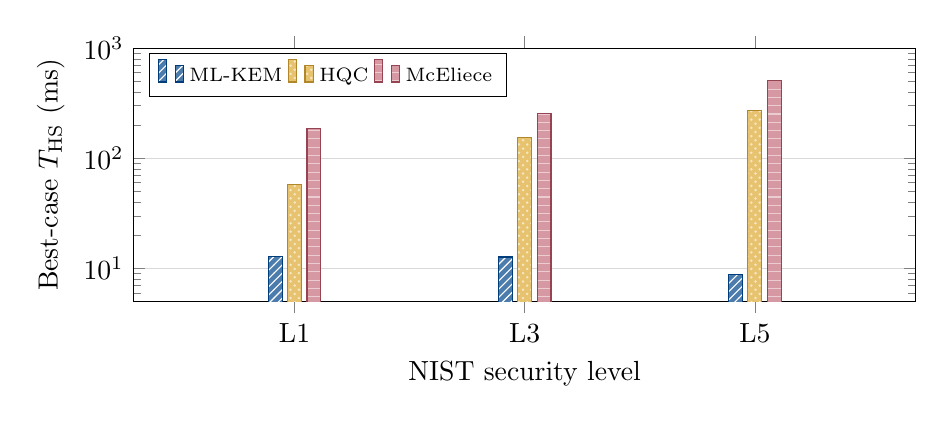
\begin{tikzpicture}
\begin{axis}[
  width=.95\columnwidth,
  height=4.8cm,
  ybar,
  bar width=5pt,
  ymode=log,
  ylabel={Best-case $T_\text{HS}$ (ms)},
  symbolic x coords={L1, L3, L5},
  xtick=data,
  xlabel={NIST security level},
  ymin=5, ymax=1000,
  legend style={at={(0.02,0.98)},anchor=north west,font=\scriptsize,
    legend columns=3},
  ymajorgrids=true,
  enlarge x limits=0.35,
]
\addplot[fill=ptblue!70, draw=ptblue!90!black,
  postaction={pattern=north east lines, pattern color=white}]
  coordinates {(L1,12.80) (L3,12.71) (L5,8.75)};
\addplot[fill=ptgold!70, draw=ptgold!80!black,
  postaction={pattern=crosshatch dots, pattern color=ptgold!30}]
  coordinates {(L1,57.80) (L3,155.8) (L5,271.7)};
\addplot[fill=ptrose!60, draw=ptrose!80!black,
  postaction={pattern=horizontal lines, pattern color=ptrose!30}]
  coordinates {(L1,187.5) (L3,257.4) (L5,505.3)};
\legend{ML-KEM, HQC, McEliece}
\end{axis}
\end{tikzpicture}
\caption{Best-case measured handshake time per KEM family and NIST
  level (fastest SIG pairing, log scale).  ML-KEM achieves
  $<$\,13\,ms at all levels; McEliece exceeds 500\,ms at L5.}
\label{fig:suite_hs}
\end{figure}

\begin{table*}[t]
\centering
\caption{Measured End-to-End Suite Handshake Performance --- All 24 Level-Matched KEM$\times$SIG Combinations (Baseline, No DDoS Detector)}
\label{tab:suite}
\footnotesize
\begin{tabular}{@{}llrrrrrl@{}}
\toprule
\textbf{KEM} & \textbf{SIG} &
  \textbf{$T_\text{HS}$} &
  \textbf{$T_\text{crypto}$} &
  \textbf{$\hat{E}_\text{HS}$} &
  \textbf{Crypto} &
  \textbf{$\rho$} & \textbf{Viable?} \\
& & (ms) & (ms) & (mJ) & (\%) & & \\
\midrule
\multicolumn{8}{@{}l}{\textit{NIST Level 1 \normalfont(3~KEMs $\times$ 3~SIGs = 9 suites)}} \\
ML512  & F512   &     12.80 &     5.69 &   44.3 &  44 & 1.0$\times$ & \checkmark \\
ML512  & DSA44  &     14.34 &     2.45 &   49.6 &  17 & 1.1$\times$ & \checkmark \\
HQ128  & F512   &     57.80 &    54.30 &  200   &  94 & 4.5$\times$ & \checkmark \\
HQ128  & DSA44  &     61.43 &    56.50 &  213   &  92 & 4.8$\times$ & \checkmark \\
MC348  & DSA44  &    187.5  &   132.3  &  649   &  71 & 14.6$\times$ & \checkmark$^\star$ \\
MC348  & F512   &    206.1  &   161.4  &  713   &  78 & 16.1$\times$ & \checkmark$^\star$ \\
ML512  & SP128  &    655.1  &   644.8  & 2\,268 &  98 & 51.2$\times$ & $\times$ \\
HQ128  & SP128  &    722.8  &   718.1  & 2\,502 &  99 & 56.5$\times$ & $\times$ \\
MC348  & SP128  &  1\,080   & 1\,045   & 3\,739 &  97 & 84.3$\times$ & $\times$ \\
\midrule
\multicolumn{8}{@{}l}{\textit{NIST Level 3 \normalfont(3~KEMs $\times$ 2~SIGs = 6 suites)}} \\
ML768  & DSA65  &     12.71 &     2.71 &   44.3 &  21 & 1.0$\times$ & \checkmark \\
HQ192  & DSA65  &    155.8  &   159.9  &  543   & 100$^\ddagger$ & 12.3$\times$ & \checkmark$^\star$ \\
MC460  & DSA65  &    257.4  &   185.4  &  897   &  72 & 20.2$\times$ & \checkmark$^\star$ \\
ML768  & SP192  &  1\,250   & 1\,233   & 4\,362 &  99 & 98.3$\times$ & $\times$ \\
HQ192  & SP192  &  1\,537   & 1\,533   & 5\,364 & 100 & 120.9$\times$ & $\times$ \\
MC460  & SP192  & 48\,186$^\dagger$ & ---  & ---   & --- & ---  & $\times$ \\
\midrule
\multicolumn{8}{@{}l}{\textit{NIST Level 5 \normalfont(3~KEMs $\times$ 3~SIGs = 9 suites)}} \\
ML1024 & F1024  &      8.75 &     1.82 &   30.5 &  21 & 1.0$\times$ & \checkmark \\
ML1024 & DSA87  &     16.78 &     2.25 &   58.5 &  13 & 1.9$\times$ & \checkmark \\
HQ256  & F1024  &    271.7  &   283.7  &  947   & 100$^\ddagger$ & 31.1$\times$ & \checkmark$^\star$ \\
HQ256  & DSA87  &    276.1  &   288.9  &  963   & 100$^\ddagger$ & 31.6$\times$ & \checkmark$^\star$ \\
MC8192 & DSA87  &    505.3  &   367.3  & 1\,763 &  73 & 57.7$\times$ & $\times$ \\
MC8192 & F1024  &    678.4  &   527.9  & 2\,367 &  78 & 77.5$\times$ & $\times$ \\
ML1024 & SP256  &  1\,110   & 1\,092   & 3\,873 &  98 & 126.9$\times$ & $\times$ \\
HQ256  & SP256  &  1\,470   & 1\,494   & 5\,128 & 100$^\ddagger$ & 168.0$\times$ & $\times$ \\
MC8192 & SP256  &  1\,651   & 1\,525   & 5\,759 &  92 & 188.7$\times$ & $\times$ \\
\bottomrule
\end{tabular}
\begin{tablenotes}
\footnotesize
\item $T_\text{HS}$: measured end-to-end handshake time.
  $T_\text{crypto}$: sum of in-suite KEM and SIG primitive times.
  $\hat{E}_\text{HS}$: estimated energy ($P_\text{avg} \times T_\text{HS}$, using
    per-primitive power from Tables~\ref{tab:kem}--\ref{tab:sig}).
  $\rho$: relative to fastest suite at same NIST level.
  Viable: \checkmark\,$T_\text{HS} < 100$\,ms;
  $\checkmark^\star$\,extended rekey;
  $\times$\,$T_\text{HS} > 500$\,ms or timeout.
  $^\dagger$Timeout at 48.2\,s; crypto fields unavailable.
  $^\ddagger$$T_\text{crypto} > T_\text{HS}$ (measurement jitter); capped at 100\%.
\end{tablenotes}
\end{table*}

The default suite (ML768+DSA65) completes a full handshake in
12.71\,ms at Level~3, of which only 2.71\,ms (21\%) is
cryptographic computation; the remaining $\sim$10\,ms comprises
protocol framing, HKDF derivation, and interpreter overhead.
ML1024+F1024 at Level~5 measures 8.75\,ms---the fastest of all
24 suites---because Falcon-1024's combined sign+verify (1.18\,ms)
undercuts ML-DSA-65 (1.94\,ms).

Three structural findings emerge: (1)~ML-KEM suites are the only
family achieving sub-100\,ms handshakes at every level
($\rho \leq 1.9\times$); (2)~SPHINCS$^+$ renders any suite
non-viable regardless of KEM choice ($T_\text{HS} \geq 655$\,ms);
(3)~McEliece at L5 exceeds 500\,ms due to keygen asymmetry.  The
MC460+SP192 timeout at 48.2\,s empirically justifies the
scheduler's constraint forbidding McEliece$\times$SPHINCS$^+$ pairs.

\emph{Takeaway: Protocol overhead dominates crypto cost for
lattice-based suites; ML-KEM$\times$ML-DSA/Falcon handshakes
complete under 17\,ms through NIST Level~5.}

% =====================================================================
\subsection{Data-Plane AEAD Performance}
\label{sec:aead}

AEAD selection operates on the UDP data plane and does \emph{not}
affect handshake timing.  Table~\ref{tab:aead} reports results from
10\,000 iterations (500 warmup, two-pass methodology: timing with
GC disabled, power with INA219 at $\sim$\,100\,Hz).

\begin{table}[t]
\centering
\caption{AEAD Performance at 256-Byte Payload (10\,000 iter, RPi4).
  Independent verification run; native~C Ascon-128a backend
  (ascon-c v1.2 opt64).}
\label{tab:aead}
\footnotesize
\begin{tabular}{@{}lrrrrrr@{}}
\toprule
\textbf{Cipher} &
  \textbf{Enc} & \textbf{Dec} &
  \textbf{$P_\text{enc}$} & \textbf{$P_\text{dec}$} &
  \textbf{$E_\text{pkt}$} & \textbf{$E_\text{bit}$} \\
& ($\mu$s) & ($\mu$s) & (W) & (W) & ($\mu$J) & (nJ/bit) \\
\midrule
AESG & 9.25  & 9.09  & 3.63 & 3.57 & 66.0  & 32.2 \\
CH20 & 6.47  & 6.05  & 3.54 & 3.58 & 44.6  & 21.8 \\
ASC  & 12.72 & 12.85 & 3.84 & 3.59 & 95.0  & 46.4 \\
\bottomrule
\end{tabular}
\begin{tablenotes}
\footnotesize
\item $E_\text{pkt} = P_\text{avg} \times (t_\text{enc} + t_\text{dec})$.
  $E_\text{bit} = E_\text{pkt} / 2048$.
  Board-level power ($P_\text{idle} = 3.320$\,W not subtracted).
  $\Delta P$ above idle: AESG\,0.31, CH20\,0.22, ASC\,0.52\,W.
\end{tablenotes}
\end{table}

Timing is concentrated ($\sigma_\text{enc}$: AESG\,0.38\,$\mu$s,
ASC\,0.77\,$\mu$s).
CH20 exhibits $\sigma = 3.99$\,$\mu$s from rare scheduling jitter
(P95\,=\,6.46, P99\,=\,6.69\,$\mu$s; median 6.30\,$\mu$s).

Fig.~\ref{fig:aead_scaling} shows latency scaling from MAVLink
telemetry (9\,B) to bulk transfer (4096\,B).

\begin{figure}[t]
\centering
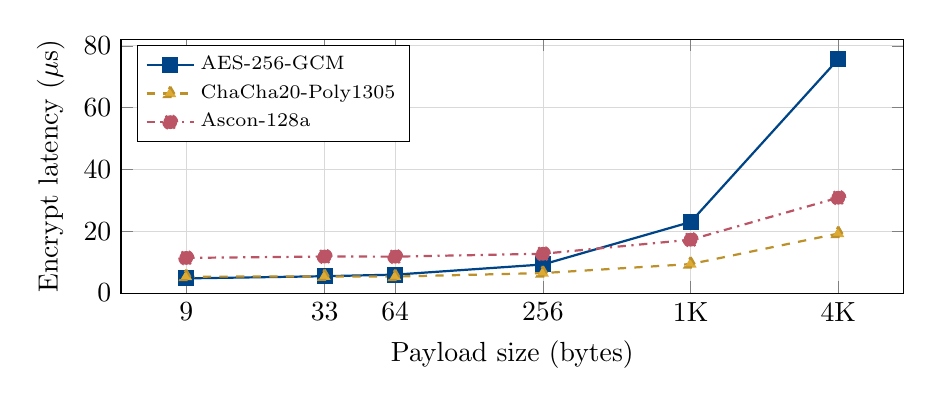
\begin{tikzpicture}
\begin{axis}[
  width=.95\columnwidth,
  height=4.8cm,
  xlabel={Payload size (bytes)},
  ylabel={Encrypt latency ($\mu$s)},
  xmode=log,
  log basis x=2,
  xtick={9,33,64,256,1024,4096},
  xticklabels={9,33,64,256,1K,4K},
  ymin=0, ymax=82,
  legend style={at={(0.02,0.98)},anchor=north west,font=\scriptsize},
  ymajorgrids=true,
  xmajorgrids=true,
  every axis plot/.append style={thick},
  mark size=2.5pt,
]
% AESG - solid + square markers
\addplot[ptblue, mark=square*, mark options={fill=ptblue}]
  coordinates {(9,4.75)(33,5.45)(64,5.96)(256,9.25)(1024,22.98)(4096,75.71)};
% CH20 - dashed + triangle markers
\addplot[ptgold!85!black, mark=triangle*, dashed, mark options={fill=ptgold}]
  coordinates {(9,5.30)(33,5.38)(64,5.33)(256,6.47)(1024,9.38)(4096,19.25)};
% ASC - dashdotted + circle markers
\addplot[ptrose, mark=*, dashdotted, mark options={fill=ptrose}]
  coordinates {(9,11.38)(33,11.82)(64,11.78)(256,12.72)(1024,17.27)(4096,30.86)};
\legend{AES-256-GCM, ChaCha20-Poly1305, Ascon-128a}
\end{axis}
\end{tikzpicture}
\caption{AEAD encrypt latency versus payload size.  ChaCha20 (NEON
  SIMD) scales at 3.4\,$\mu$s/KiB; AES-GCM at 17.7\,$\mu$s/KiB
  (software table-lookup).  Below 64\,B, setup cost dominates and
  ciphers converge.}
\label{fig:aead_scaling}
\end{figure}

At 4096\,B, CH20 is 3.93$\times$ faster than AESG due to NEON
vectorization versus software AES table lookups.  Below 64\,B,
setup cost dominates and the ciphers converge.  Energy per bit at
256\,B: CH20\,=\,21.8, AESG\,=\,32.2, ASC\,=\,46.4\,nJ/bit.
For a 50\,Hz MAVLink stream ($\sim$\,256\,B packets), per-second
AEAD cost ranges from 2.23\,mJ (CH20) to 4.75\,mJ (ASC)---negligible
versus the 3.32\,W board draw.

\emph{Takeaway: ChaCha20-Poly1305 delivers 32\% lower energy per
bit than AES-256-GCM on Cortex-A72 without hardware AES, making it
the optimal data-plane cipher for this platform.}

% =====================================================================
\subsection{Adversarial Interaction Impact}
\label{sec:ddos}

Concurrent DDoS detection competes with the cryptographic pipeline
for CPU and thermal headroom.  All 72 level-matched suites were
benchmarked under baseline (no detector), XGBoost, and TST scenarios
(10\,s per suite per scenario).%
\footnote{XGBoost: 15\,000 trees, 54~features, 15~CIC-IoT-2023
  classes; TST: Time-Series Transformer, \texttt{seq\_len=1}
  (functionally a 3-layer MLP), 1.6\,M parameters, 46~features,
  6~coarse classes.}

Table~\ref{tab:detector_compare} presents a head-to-head comparison
of XGBoost and TST across accuracy, resource, and handshake-impact
dimensions.  Fig.~\ref{fig:cross_axis} visualises the cross-axis
cost interactions.  Default-suite values are for ML768+DSA65+AESG.

\begin{table}[t]
\centering
\caption{XGBoost vs.\ TST Head-to-Head on RPi4 (CIC-IoT-2023)}
\label{tab:detector_compare}
\footnotesize
\setlength{\tabcolsep}{3.5pt}
\begin{tabular}{@{}lrrr@{}}
\toprule
\textbf{Metric} & \textbf{XGBoost} & \textbf{TST} & \textbf{Ratio} \\
\midrule
\multicolumn{4}{@{}l}{\textit{Detection quality}} \\
Accuracy (\%)               & 94.55  & 90.27  & ---        \\
F1-macro                     & 0.947  & 0.80   & ---        \\
\midrule
\multicolumn{4}{@{}l}{\textit{Inference cost (isolated, 15\,s run)}} \\
$t_\text{inf}$ mean (ms)    & 7.42   & 10.72  & 1.44$\times$ \\
$t_\text{inf}$ P99 (ms)     & 9.52   & 26.12  & 2.74$\times$ \\
Throughput (pred/s)          & 134.6  & 93.2   & 0.69$\times$ \\
$E_\text{inf}$ (mJ)         & 31.7   & 56.7   & 1.79$\times$ \\
\midrule
\multicolumn{4}{@{}l}{\textit{System impact (default suite)}} \\
CPU avg / peak (\%)          & 40.2\,/\,61.4 & 87.8\,/\,94.1 & 2.2$\times$\,/\,1.5$\times$ \\
$\Delta P$ above idle (mW)  & +951   & +1\,973 & 2.07$\times$ \\
$\Delta T$ (${^\circ}$C)    & +14.1  & +21.9  & 1.55$\times$ \\
$T_\text{HS}$ (ms)          & 13.46  & 37.90  & 2.82$\times$ \\
HS overhead vs.\ baseline   & +3.5\% & +191\% & 55$\times$   \\
\bottomrule
\end{tabular}
\begin{tablenotes}
\footnotesize
\item Idle baseline: $P_\text{idle}=3.309$\,W,
  CPU\,14.7\%, $T_\text{HS}^\text{base}=13.01$\,ms.
  CPU peak: max observed during 72-suite sweep.
  $\Delta T$: rise over baseline for default suite (10\,s run).
\end{tablenotes}
\end{table}

\begin{figure}[t]
\centering
\begin{subfigure}[b]{\columnwidth}
\centering
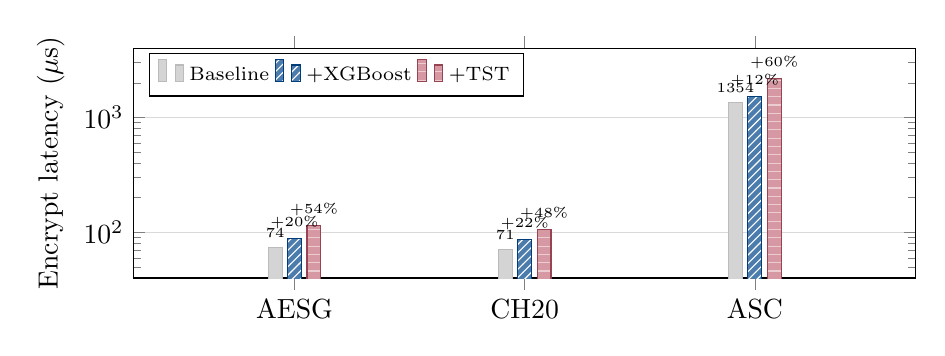
\begin{tikzpicture}
\begin{axis}[
  width=.95\columnwidth,
  height=4.5cm,
  ybar,
  bar width=5pt,
  ymode=log,
  ylabel={Encrypt latency ($\mu$s)},
  symbolic x coords={AESG, CH20, ASC},
  xtick=data,
  ymin=40, ymax=4000,
  legend style={at={(0.02,0.98)},anchor=north west,font=\scriptsize,
    legend columns=3},
  ymajorgrids=true,
  enlarge x limits=0.35,
  nodes near coords,
  point meta=explicit symbolic,
  every node near coord/.append style={font=\tiny,anchor=south},
]
% Baseline (no detector)
\addplot[fill=ptgray!50, draw=ptgray!80]
  coordinates {
    (AESG, 73.8) [{74}]
    (CH20, 71.2) [{71}]
    (ASC, 1353.7) [{1354}]
  };
% +XGBoost
\addplot[fill=ptblue!70, draw=ptblue!90!black,
  postaction={pattern=north east lines, pattern color=white}]
  coordinates {
    (AESG, 88.9) [{+20\%}]
    (CH20, 86.8) [{+22\%}]
    (ASC, 1510.5) [{+12\%}]
  };
% +TST
\addplot[fill=ptrose!60, draw=ptrose!80!black,
  postaction={pattern=horizontal lines, pattern color=ptrose!30}]
  coordinates {
    (AESG, 113.9) [{+54\%}]
    (CH20, 105.3) [{+48\%}]
    (ASC, 2165.9) [{+60\%}]
  };
\legend{Baseline, +XGBoost, +TST}
\end{axis}
\end{tikzpicture}
\caption{DDoS\,$\to$\,AEAD: per-packet encrypt latency under
  concurrent detection (72-suite campaign mean, log scale).
  Labels show absolute $\mu$s (baseline) or overhead~\%.
  All three ciphers degrade; TST imposes 48--60\% overhead.}
\label{fig:ddos_to_aead}
\end{subfigure}
\vspace{2pt}
\begin{subfigure}[b]{\columnwidth}
\centering
\resizebox{\columnwidth}{!}{%
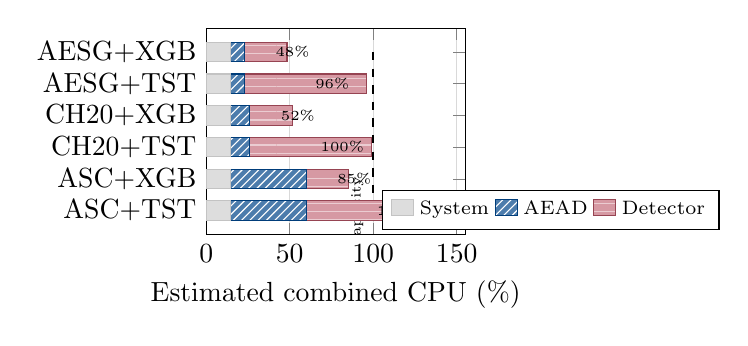
\begin{tikzpicture}
\begin{axis}[
  height=4.2cm,
  xbar stacked,
  bar width=7pt,
  xlabel={Estimated combined CPU (\%)},
  symbolic y coords={
    {ASC+TST},
    {ASC+XGB},
    {CH20+TST},
    {CH20+XGB},
    {AESG+TST},
    {AESG+XGB}},
  ytick=data,
  xmin=0, xmax=155,
  xmajorgrids=true,
  ymajorgrids=false,
  enlarge y limits=0.15,
  legend style={at={(0.68,0.02)},anchor=south west,font=\scriptsize,
    legend columns=3},
]
% Layer 1: System idle (14.7% for all)
\addplot[fill=ptgray!40, draw=ptgray!70]
  coordinates {
    (14.7,{AESG+XGB}) (14.7,{AESG+TST})
    (14.7,{CH20+XGB}) (14.7,{CH20+TST})
    (14.7,{ASC+XGB})  (14.7,{ASC+TST})
  };
% Layer 2: AEAD cipher CPU
\addplot[fill=ptblue!70, draw=ptblue!90!black,
  postaction={pattern=north east lines, pattern color=white}]
  coordinates {
    (8.2,{AESG+XGB})  (8.2,{AESG+TST})
    (11.4,{CH20+XGB}) (11.4,{CH20+TST})
    (45.2,{ASC+XGB})  (45.2,{ASC+TST})
  };
% Layer 3: Detector CPU
\addplot[fill=ptrose!60, draw=ptrose!80!black,
  postaction={pattern=horizontal lines, pattern color=ptrose!30},
  nodes near coords,
  point meta=explicit symbolic,
  every node near coord/.append style={font=\tiny,anchor=west}]
  coordinates {
    (25.5,{AESG+XGB}) [{48\%}]
    (73.1,{AESG+TST}) [{96\%}]
    (25.5,{CH20+XGB}) [{52\%}]
    (73.1,{CH20+TST}) [{100\%}]
    (25.5,{ASC+XGB})  [{85\%}]
    (73.1,{ASC+TST})  [{\textbf{133\%}}]
  };
% 100% capacity line
\draw[ptblack, thick, dashed]
  (axis cs:100,{AESG+XGB}) -- (axis cs:100,{ASC+TST});
\node[font=\tiny,ptblack,anchor=south,rotate=90]
  at (axis cs:100,{ASC+TST}) {capacity};
\legend{System, AEAD, Detector}
\end{axis}
\end{tikzpicture}}% end resizebox
\caption{AEAD\,$\to$\,DDoS: estimated CPU breakdown for each
  cipher$\times$detector pair.  System idle = 14.7\%; AEAD and
  detector portions are additive.  ASC+TST exceeds single-core
  capacity (dashed line)---forbidden by MDEAS.}
\label{fig:aead_to_ddos}
\end{subfigure}
\caption{Bidirectional AEAD$\leftrightarrow$DDoS cross-axis
  interaction.  (a)~Detector CPU contention inflates per-packet
  AEAD latency by 12--22\% (XGBoost) to 48--60\% (TST).
  (b)~Heavy ciphers consume the headroom needed by detectors;
  only AES-GCM and ChaCha20 leave sufficient budget for both
  detector types.}
\label{fig:cross_axis}
\end{figure}

Fig.~\ref{fig:cross_axis} reveals a fundamental asymmetry in the
three-axis interaction structure.  Four cross-axis directions exist;
their magnitudes differ by three orders of magnitude.

\medskip
\textbf{DDoS\,$\to$\,PQC (handshake contention).}\quad
Concurrent detection inflates the default-suite handshake:
$T_\text{HS}$ rises from 13.01\,ms (baseline) to 13.46\,ms
(+3.5\%) with XGBoost and 37.90\,ms (+191\%) with TST
(Table~\ref{tab:detector_compare}).  Across all 72 suites, XGBoost
adds mean~+2.5\% / median~+0.05\% (max~+137.2\%); TST
adds mean~+71.8\% / median~+32.6\% (max~+405.1\%).  However,
PQC handshakes occupy $<$\,0.05\% of each 30\,s rekey cycle
($\Phi < 5 \times 10^{-4}$, Eq.~\ref{eq:rekey}), so this penalty
is transient.

\medskip
\textbf{DDoS\,$\to$\,AEAD (data-plane contention).}\quad
This is the \emph{dominant} cross-axis cost because both subsystems
run continuously.  Fig.~\ref{fig:ddos_to_aead} and
Table~\ref{tab:aead_cross} report per-packet encrypt latency under
concurrent detector load (72-suite campaign mean).
XGBoost imposes 12--22\% overhead across all three ciphers;
TST imposes 48--60\%.  The log-scale grouping in
Fig.~\ref{fig:ddos_to_aead} reveals that Ascon's baseline latency
(1\,354\,$\mu$s) already exceeds AES-GCM's worst-case under TST
(114\,$\mu$s) by 12$\times$, compounding the cross-axis penalty.

\begin{table}[t]
\centering
\caption{AEAD Encrypt Latency Under Concurrent DDoS Detection
  (72-Suite Campaign Mean, RPi4)}
\label{tab:aead_cross}
\footnotesize
\setlength{\tabcolsep}{3pt}
\begin{tabular}{@{}lrrrr@{}}
\toprule
\textbf{Cipher} &
  \textbf{Baseline} & \textbf{+XGB} & \textbf{+TST} &
  \textbf{TST\,/\,Base} \\
& ($\mu$s) & ($\mu$s) & ($\mu$s) & \\
\midrule
AESG & 73.8  & 88.9\,(+20\%)  & 113.9\,(+54\%) & 1.54$\times$ \\
CH20 & 71.2  & 86.8\,(+22\%)  & 105.3\,(+48\%) & 1.48$\times$ \\
ASC  & 1\,353.7 & 1\,510.5\,(+12\%) & 2\,165.9\,(+60\%) & 1.60$\times$ \\
\bottomrule
\end{tabular}
\begin{tablenotes}
\footnotesize
\item Values from \texttt{analysis\_deep\_dive.csv}.
  ASC measured with pure-Python backend as deployed during the
  DDoS campaign; native~C backend (Table~\ref{tab:aead}) is
  100$\times$ faster but was not used in this cross-axis campaign.
  Ascon is forbidden under both detectors by the MDEAS.
\end{tablenotes}
\end{table}

\textbf{AEAD\,$\to$\,DDoS (CPU headroom).}\quad
Fig.~\ref{fig:aead_to_ddos} decomposes the CPU budget into system,
AEAD, and detector contributions.  At 50\,Hz MAVLink: AES-GCM uses
8.2\%, ChaCha20 11.4\%, and Ascon 45.2\% CPU.  XGBoost adds
$\sim$25.5\% and TST $\sim$73.1\% above system idle.
Combined, Ascon+TST would demand $\sim$133\% CPU---crossing the
single-core capacity line (Fig.~\ref{fig:aead_to_ddos}, dashed).
Even Ascon+XGBoost reaches 85\%, leaving negligible thermal margin.
The MDEAS therefore forbids Ascon under TST and flags it as
marginal under XGBoost at rates $>$\,200\,Hz.

\textbf{PQC\,$\to$\,DDoS (rekey burst).}\quad
During the 13\,ms ML-KEM handshake, no inference runs; but
$\Phi(30\,\text{s}) < 0.05\%$ (Eq.~\ref{eq:rekey}), so the
detection gap is one missed sample at 100\,Hz---negligible.
McEliece keygen (up to 9\,s) would block inference for an
extended window, reinforcing the ML-KEM preference.

\emph{Takeaway: The dominant cross-axis penalty is
DDoS$\leftrightarrow$AEAD because both run continuously.
PQC interactions are transient ($\Phi < 0.05\%$) for ML-KEM
suites.  XGBoost is the only viable detector: it limits AEAD
overhead to 20--22\% at 4.3\,pp higher accuracy than TST.}

% =====================================================================
\subsection{Scheduler Implications}
\label{sec:scheduler}

The Multi-Dimensional Energy-Aware Scheduler (MDEAS) manages three
decision axes at 1\,Hz: AEAD cipher selection, security-level
promotion/demotion (triggering PQC rekey), and DDoS detector
activation.  Each level transition requires a full handshake.
The rekey overhead fraction is:
\begin{equation}
\Phi(R) = \frac{T_\text{HS}}{R + T_\text{HS}}
\label{eq:rekey}
\end{equation}
where $R$ is the rekey interval.  For the default suite
($T_\text{HS} = 12.71$\,ms) at the minimum 30\,s interval:
$\Phi = 4.2 \times 10^{-4}$ ($<$0.05\%).  Even ML768+SP192
($T_\text{HS} = 1.25$\,s) at 30\,s yields $\Phi = 0.040$
(4.0\%).

Table~\ref{tab:detector_overhead} maps each detector state to the
thermal activation ceiling used by the MDEAS.

\begin{table}[t]
\centering
\caption{MDEAS Detector Thermal Activation Ceilings}
\label{tab:detector_overhead}
\footnotesize
\begin{tabular}{@{}lrrrr@{}}
\toprule
\textbf{Detector} &
  \textbf{$\Delta P$} & \textbf{$\Delta T$} &
  \textbf{CPU peak} & \textbf{$T_\text{max}$} \\
& (W) & ($^\circ$C) & (\%) & ($^\circ$C) \\
\midrule
None    & 0.00 & 0.0  & 36.5  & 80.0 \\
XGBoost & 0.95 & 14.1 & 61.4  & 65.9 \\
TST     & 1.97 & 21.9 & 94.1  & 58.1 \\
\bottomrule
\end{tabular}
\begin{tablenotes}
\footnotesize
\item $T_\text{max} = 80^\circ\text{C} - \Delta T$: temperature
  ceiling before activation is blocked.
  $\Delta T$, CPU peak from default-suite measurements
  (Table~\ref{tab:detector_compare}).
\end{tablenotes}
\end{table}

Cross-axis constraints prevent pathological configurations:
Ascon-128a is forbidden under TST (per-packet cost plus 93\% CPU
exceeds the real-time budget); McEliece$\times$SPHINCS$^+$ pairs
are forbidden ($T_\text{HS}$ exceeds the 45\,s rekey timeout);
detector activation is blocked above the per-detector $T_\text{max}$.
These constraints reduce 648 theoretical configurations
(216~suites $\times$ 3~detector states) to $\sim$500 viable
operating points.

\emph{Takeaway: Rekey overhead is negligible ($<$\,0.05\%) for
ML-KEM suites.  The MDEAS navigates the security--energy--thermal
Pareto surface via 1\,Hz telemetry while guaranteeing the
configured minimum security level.}


\end{document}
